% !TeX root = surgery.tex
\subsection{The Nepalese Version}

In the present article and other publications of our research group, we focus on the study of what we call the `Nepalese version' of the \SS. The primary rationale behind using this designation was outlined in \citet[2-3]{kleb-2021b}, but but we consider it necessary to reflect upon its meaning here given the conceptual significance that this term occupies in our research.
%, given the conceptual significance that this term occupies in our research, we consider it necessary to reflect upon its meaning here.\q{suggestion: but we consider it necessary to reflect upon its meaning here given the conceptual significance that this term occupies in our research.} 
It is likely that in the course of our research, we will refine our understanding of the phenomenon and, consequently, review and modify our current interpretation.%\q{is it sufficient to say 'our current interpretation'?}

Put plainly, the `Nepalese version' refers to a hypothetical text-critical reconstruction of the wording of the \SS\ that is based primarily on the evidence of three ancient Nepalese manuscripts, which we have briefly introduced above and which we will describe in more detail in a later section.  We call these MSS `Nepalese' not just because they were preserved and discovered by modern scholarship 
%to\q{discovered by modern scholarship} the modern scholarship 
in the 
%present-day 
Kathmandu valley
%\q{seeing that you say 'modern scholarship', 'present-day' seems redundant} 
but also because we believe that they were produced in the same area. We conclude this because all three MSS are written in a specific variety of Indic scripts, which, to the best of our knowledge, was not used outside of the region. 

Furthermore, we speak of a single `version' because we hold that these manuscripts attest to a peculiar line of transmission of the text, that is, in terms of stemmatic analysis, they share
%\q{they share [...] while as the same time, bear [...]} 
a common ancestor (hyparchetype) or a group of ancestors, while at the same time, bear no signs of significant contamination. This hypothesis was postulated in \citet{kleb-2010} and reiterated in \citet{kleb-2021a} as the result of a systematic analysis of two complete chapters (SS.1.3 and SS.1.15)
%\q{So far we have been using SS.1.3 format} 
as well as several shorter excerpts from the \SS\ transmitted in the Nepalese manuscripts. 
On the one hand, these studies highlight that all three MSS preserve a highly uniform text with very few variations, virtually all of which can be explained as standard scribal errors or corrections. 
On the other hand, \citet{kleb-2010,kleb-2021a} has systematically compared
%systematically compare\q{has systematically compared (the subject is singular)} 
the concerned textual excerpts with four printed editions, alternative readings (\emph{pāṭha}s) reported by several commentators,
%the \q{several commentators? as the list is not exhaustive}commentators (two medieval authors, Cakrapāṇidatta and Ḍalhaṇa, as well as an early modern Bengali scholar Haraṇacandra), 
parallel passages in other texts, and, only sporadically, with a few additional manuscripts of the \SS. This analysis demonstrates that the text of the \SS\ preserved in the Nepalese MSS differs decidedly from all the above standards of comparison. In this way, for example, we establish that another Nepalese manuscript of the \SS, NAK 1-1146,%
    \footnote{%
    See 
    \url{http://ngmcp.fdm.uni-hamburg.de/mediawiki/index.php/A_224-9_Suśrutasaṃhitā}
     (accessed on November 8, 2021).%
    } 
does not belong to the peculiar line of textual transmission and need not be taken into consideration when reconstructing the reading of its hyparchetype. 
However, \q{new paragraph?} in view of the vast number of handwritten copies of the \SS\ preserved in different libraries across South Asia and in the absence of their systematic inclusion into the project's current collation,
%collation\q{the project's current collation}, 
the assumption about the regional character of the transmission line remains purely hypothetical. As a matter of fact, we believe that the Nepalese MSS preserve many original features of the \SS and it is possible, even likely, that some of these features will be found in other manuscripts of this work that have yet to be studied.%, particularly in those that contain versions that differ from that propagated by Ḍalhaṇa.
%As a matter of fact, we believe that the Nepalese MSS preserve many original features of the \SS, and as such, these are likely attested in other textual witnesses as well.\q{I'm not sure of the intended meaning here. Is some contrast intended (i.e., although we believe that [...], many of the same features are likely attested in textual witnesses from other regions as well)?}

Our research group builds upon the above hypothesis about the existence of a distinct Nepalese version of the \SS and concentrates primarily on the study of this text in its own right and, additionally, in comparison to a single version of the compendium popularized by its late medieval commentator Ḍalhaṇa and recorded in the widely used \cite{vulgate}. Nevertheless, the present study of SS.1.16 also considers the readings found in \cite{acar-1939} and incorporates various observations made by both medieval commentators (Cakrapāṇidatta and Ḍalhaṇa) into the notes of the edition and some annotations of the translation.
%\q{We also looked at Cakrapāṇi and incorporated his comments into the notes of the edition and some annotations of the translation. Perhaps, here, you means to say, 'builds upon the above hypothesis by a detailed comparison of 1.16 of the Nepalese version with the version popularized by its late medieval commentator Ḍalhaṇa [...]}

The current paper and several earlier publications%
    \footnote{%
    See, for example, \citet{hari-2011}, \citet{wuja-2013}, \citet{birc-2021}, \citet{birc-2021a}.%
    } 
furnish a vast catalogue of uniform features, which are characteristic of the Nepalese MSS and set them apart from the text known from\q{known as} the vulgate version. These features of the Nepalese MSS pertain to orthographic variants, peculiarities in the structure and structuring elements, as well as the actual wording of the text. As argued elsewhere in this article, many of these variants are likely to be closer to the original, not just because they preserve what appears to be a less edited, that is, less understandable,\q{[...], that is, a less easily understood, [...]} version of the text, and thus invoke the principle \emph{lectio difficilior potior}.\q{I'm not too sure of the meaning of the last phrase. Is 'invoking this principle' a reason for these  variants being likely closer to the original? Maybe you mean something like, [...] text, which suggests it was closer to the original according to the principle of \emph{lectio difficilior potior}.}

We\q{I'd drop the  'not just because' in the previous sentence. If you retain it, you need something at the beginning of the next sentence to link to it, such as [not just because ...]. On the contrary [...]. Both reasons are important, so you could just say,'many of these variants are likely to be closer to the original for two reasons. Firstly, [...]. Secondly and more importantly, [...] } assign a high value to many Nepalese readings mainly because they constitute internally more consistent and coherent text that is at times further supported by external sources.\q{an internally [...]}

Additionally, we want to highlight that we do not think that the Nepalese MSS attest to the original text of the \SS. On the contrary, in reconstructing the Nepalese version, we occasionally make use of corrections and emendations, and, as far as the reconstructed text is concerned, we believe that it bears signs of secondary editorial effort.\q{This is not clear. I think you mean to say that the Nepalese mss attest to a hyparchetype rather than the archetype of the \SS. Our use of emendations and corrections is not proof of this, because these methods are needed whether we are constructing an archetype or hyparchetype. Signs of past redactors editing the text is possible proof (and do you have refs or examples?) but such signs might also be the result of an author's attempt to compile older materials. The point you make below about the colophons strikes me as more of a scribal issue rather than authorial one.}
Nevertheless, we think that the Nepalese MSS provide a unique opportunity for assessing a single line of textual transmission that goes back to a hyparchetype, which likely predates the composition of all major commentaries on the \SS, and that, due to its regional character, has suffered relatively little contamination. The hypothetical readings of this hyparchetype we term the `Nepalese version'. 
%When evaluating these readings historically, it is further necessary to keep in mind that there is plentiful evidence suggesting an ancient age of the readings accepted into Ḍalhaṇa’s version of the text. 


\subsection{Cakrapāṇidatta and Ḍalhaṇa's Versions}
The commentaries of Cakrapāṇidatta and Ḍalhaṇa, called the \emph{Bhānumatī} and \emph{Nibandhasaṅgraha} respectively, are based on similar versions of the \SS, both of which are significantly different to the Nepalese version. Ḍalhaṇa was aware of Cakrapāṇidatta's work and reiterated many of his predecessor's remarks, so the commentator's interpretation of the root text is largely consistent. 

Trikamajī Ācārya's edition of the \textit{Sūtrasthāna} of the \emph{Bhānumatī} \citep{acar-1939} duplicates the version of the \SS\ in his edition of the \emph{Nibandhasaṅgraha} \citep{vulgate}, except in a few obvious cases where Cakrapāṇidatta glosses a word or compound that is different to the one glossed by Ḍalhaṇa.\footnote{For example, in SS.1.16.18, Cakrapāṇidatta glosses \emph{rājasarṣapa} whereas Ḍalhaṇa glosses \emph{gaurasarṣapa}, and Ācārya reflects this in the root texts of the \emph{Bhānumatī} \citep[130]{acar-1939} and \emph{Nibandhasaṅgraha} \citep[79]{vulgate}.} The duplication of the root text creates the somewhat misleading impression that both commentators had an almost identical version of the \SS. However, there is evidence in SS.1.16 that this was not the case. For example, Ḍalhaṇa comments on four verses (1.16.11–14, \cite[78]{vulgate}) that Cakrapāṇidatta cites separately in his commentary \citep[128–129]{acar-1939}, introducing each one as 'some people read' (\emph{ke cit paṭhanti}). This clearly indicates that these verses were not in the version of the \SS\ upon which Cakrapāṇidatta was commenting, yet Ācārya includes them in the root text of the \emph{Bhānumatī}.

Also, Cakrapāṇidatta does not acknowledge or comment on some verses in the version of the \SS\ known to Ḍalhaṇa. Although it is possible that a commentator may not have remarked on a verse because its meaning was clear, in some cases the commentarial convention of citing the first words of a new verse or passage provides firmer ground for suspecting the absence of a verse in the root text. For example, the prose passage of SS.1.16.18 in the the \emph{Bhānumatī} \citep[130]{acar-1939}, which is SS.1.16.19 in the \emph{Nibandhasaṅgraha} \citep[79]{vulgate}, is followed by several verses that elaborate on the content of the prose passage, and both commentators introduce these verses and cite the opening words of the first verse before glossing specific terms. However, Cakrapāṇidatta does not introduce, cite or comment on the same verses as Ḍalhaṇa (SS.1.16.20–22ab, \cite[79]{vulgate}), and yet the first of the verses commented on by Ḍalhaṇa appears in the root text of Ācārya's edition of the \emph{Bhānumatī} (SS.1.16.19, \cite[130]{acar-1939}), and the others (SS.1.16.20–21ab) are included in parenthesis. A similar instance of this occurs at \emph{Bhānumatī} SS.1.16.31, where Ācārya includes a verse in parenthesis that was commented on by Ḍalhaṇa (SS.1.16.32, \cite[81]{vulgate}) but not by Cakrapāṇidatta. It appears that the manuscript on which Ācārya's edition of the \emph{Bhānumatī} was based does not include the root text.\footnote{This observation is based on the opening passage of MS 1887-1935 of the \emph{Bhānumatī}, which is transcribed in Eggling 1896: 928. The transcription has the commentary without the root text. See the section below on Ācārya's 1939 edition for details of the sources Ācārya used for this edition.} Therefore, the inclusion of SS.1.16.19–21ab and 31 in the root text of the \emph{Bhānumatī} is an unsubstantiated hypothesis. 

% Ḍalhaṇa 1.16.11–14
%The version of 1.16.11–14 known to Ḍalhaṇa \citep[78]{vulgate} has four verses (\emph{śloka}) at this point that are not in the Nepalese manuscripts. The additional verses iterate the types of joins required for ear flaps that are missing, elongated, thick, wide, etc. All four verses were probably absent in the version of the \emph{Suśrutasaṃhitā} known to Cakrapāṇidatta. He cites the verses separately in his commentary, the \emph{Bhānumatī} \citep[128–129]{acar-1939}, introducing each one as 'some people read' (\emph{ke cit paṭhanti}). However,  in Trikamajī Ācārya's edition of the \emph{Sūtrasthāna} of the \emph{Bhānumatī}, the root text is largely identical to the one commented on by Ḍalhaṇa (\cite{vulgate}), even in instances like this where Cakrapāṇidatta's commentary indicates that he was reading a different version of the \emph{Suśrutasaṃhitā}

% Ḍalhaṇa 1.16.19–20 
%Cakrapāṇidatta \citep[131]{acar-1939} does not comment on these verses, nor verse 15 of the Nepalese version, and so the version of the \emph{Suśrutasaṃhitā} known to him may not have included them.

% Ḍalhaṇa 1.16.32
 %Cakrapāṇidatta \citep[133]{acar-1939} does not comment on this additional verse, which suggests that either he did not know of it or was not inclined to accept it.
 
% Both commentators were aware of a version of the \SS\ that was similar to the Nepalese version % See blog.

In fact, there is some evidence that the Nepalese version was more similar to Cakrapāṇidatta's version than to Ḍalhaṇa's. For example, 1.16.5 of the Nepalese version begins with the compound \emph{doṣasamudayāt} whereas the version known to Ḍalhaṇa (SS.1.16.6, \cite[77]{vulgate}) inserts two compounds, \emph{kliṣṭajihmāpraśastasūcīvyadhāt} and \emph{gāḍhataravartitvāt}, before this. Cakrapāṇidatta (SS.1.16.5, \cite[126–127]{acar-1939}) begins his comment on this passage by glossing \emph{doṣasamudayāt}, which suggests that he was not aware of any compounds prior to this one. If one looks beyond SS.1.16, there are instances where the Nepalese version (1.1.28) and the root text of Cakrapāṇidatta have the same reading, which Ḍalhaṇa mentions as an alternative read by others. For example, 1.1.28 of the Nepalese version has \emph{tatrāsmiñ chāstre}, which is the reading commented on by Cakrapāṇidatta (\cite[17]{acar-1939}). However, Ḍalhaṇa  (SS.1.1.22, \cite[5]{vulgate}) comments on \emph{asmiñ chāstre} and states that others read \emph{tatrāsmiñ chāstre}. Also, in his commentary on SS.1.1.8.1, Ḍalhaṇa (\cite[5]{vulgate}) notes the variant reading \emph{ṣaṣṭyā vidhānaiḥ}, which is not in his root text but evidently was in Cakrapāṇidatta's  (SS.1.1.6, \cite[11]{acar-1939}). As discussed elsewhere (Birch 2021), the reading of \emph{ṣaṣṭyā vidhānaiḥ} is likely a corruption of \emph{ṣaṣṭyābhidhānaiḥ} in the Nepalese version (1.1.9). 

% Ḍalhaṇa was aware of the reading in the Nepalese version because he notes in his commentary on 1.16.6 \citep[77]{vulgate} that some read 'because of the accummulation of humours' rather than 'because of piercing with a painful, crooked and unrecommended needle or because of a wick that is too thick.' 

\subsection{Differences between the Nepalese and Subsequent Versions of SS.1.16}

% The structural differences between the Nepalese and subsequent versions has been discussed by \citet[27–44]{kleb-2021b}, which include the frame story,\footnote{On this topic, also see the more recent \citet{birc-2021}.} the name of the first book (\emph{Ślokasthāna}), the structuring of the text according to chapter and section colophons, and an additional passage in the \emph{Kalpasthāna}. \citet[44–55]{kleb-2021b} also makes general observations on distinct features of the Nepalese version's content and looks specifically at lists of skin lesions arising from urinary disease and vital energies. And in an effort to demonstrate the possibility of greater coherence in the Nepalese version, \citet[101–104]{hari-2011} has compared its classification of snakes with Ḍalhaṇa's version. 

% On the whole, these observations indicate that [...synopsis of general conclusions here, Andrey?...]
%% 1.16 is missing yathovāca bhagavān dhanvantariḥ|

Several differences between the text of the \SS\ as found in its multiple printed versions and as reconstructed on the basis of the Nepalese MSS have been already pointed out in previous publications. In terms of the overall organization and structuring themes and elements of the text, \citet[27f.]{kleb-2021b} lists differences in the chapter sequence, \citet{wuja-2013}, \citet[28-32]{kleb-2021b} and most recently \citet{birc-2021} and \citet[2-4]{birc-2021a} talk about variations in the frame story, \citet[32-36]{kleb-2021b} highlights the interchangeable use of two names (\emph{Ślokasthāna} and \emph{Sūtrasthāna}) of the first book of the text, and \citet[37-44]{kleb-2021b} examines another peculiarity of the Nepalese version, namely, additional verse or prose colophons found at the end of each book but also each decade of chapters of the \SS. \q{This is a complicated sentence. It might be better to use semi-colons, e.g., [...] sequence; [...] frame story; [...] of the text; [...]}

As the current paper demonstrates, many distinct features pertaining to the actual content of the Nepalese version continuously come to light as we proceed with our study of the manuscripts. Among observations made in previous literature, \citet[44-47]{kleb-2021b} makes some general remarks, along with a few arbitrary examples, and details two case studies (Ibid.:47-55). The first study deals with the list of skin lesions associated with urinary disease (\emph{pramehapiṭakā} in the Nepalese spelling), whose signs and pathogenesis are described in \emph{nidānasthāna} 6 and whose treatment is the subject of \emph{cikitsāsthāna} 12. The second study focuses on the variation in another list, that of vital energies (\emph{prāṇa}s), mentioned in \emph{śārīrasthāna} 4.\q{You could save repetition by placing this sentence before 'The discussion of the textual variant in the second case study [...] and change this sentence to 'The discussion of the textual variant in the list of vital energies also recourses [...]} The list of skin lesions exemplifies a case where the text of the \SS\ transmitted in the Nepalese MSS is internally more coherent than that commented on by Ḍalhaṇa, and where the incoherence of the latter version already had been identified by an early commentator, Gayadāsa, who, based on text-external evidence,\q{do you mean to say that Gayadāsa has text-external evidence? That how it sounds. Perhaps, omit the phrase.} effectively had proposed a textual conjecture that corresponds to the reading of the Nepalese version.%
    \footnote{%
    According to our current knowledge, KL 699 was copied before the time in which Gayadāsa flourished. This relative chronology excludes the possibility that the Nepalese version incorporates Gayadāsa's conjecture rather than transmitting an original variant.%
    }
The study at hand\q{this study?} also provides a rare example of interpolation, for which we can postulate its likely source, namely, the medical theory associated with the \textit{Carakasaṃhitā}.
The\q{new paragraph?} discussion of the textual variant in the second case study, the list of vital energies, also recourses to Gayadāsa's learned remarks. Here, the scholar commented on the reading transmitted in the Nepalese MSS as the original one and reported an alternative reading and its interpretation preferred by another ancient commentator, Jejjaṭa. It is precisely this\q{the referent of this is not so clear. 'this alternative reading'?} reading that is known to modern readers of the \SS\ from the vulgate version of the text.
Another exemplary investigation of textual variants in the Nepalese version is found in \citet[101–104]{hari-2011}.
This study looks at the classification of snakes in \emph{kalpasthāna} 4 and reveals that, compared to the versions of the \SS\ found in different printed sources, the Nepalese MSS preserve a text that is internally more consistent and coherent. 

On the whole, these observations indicate that many features of the Nepalese version of the \SS\ are likely to go back to an older state of the textual development common to other versions of the compendium. 
However, other textual peculiarities, such as the text-structuring colophons concluding every tenth chapter, are likely to have occurred within a local transmission of the text, and it is improbable that they are attested in the MSS from other regions. 
When evaluating the Nepalese readings historically, however, it is further necessary to keep in mind that there is plentiful evidence suggesting an ancient age of the readings accepted into Ḍalhaṇa's version of the text. \q{[...] suggesting that some of the readings accepted by Ḍ were ancient, if not original. (?)}


The following detailed comparison of 1.16 of the Nepalese version with Ḍalhaṇa's \emph{Nibandhasaṅgraha} unfolded as the chapter was edited. The differences appear to emanate largely from attempts to standardise, simplify or clarify the language of the Nepalese version, add and redact information, and introduce changes to recipes and treatments. Examples from 1.16 have been provided to demonstrate the general observations which, it is hoped, a larger survey of the text will verify.

Table 1 reveals the extent to which 1.16 of the Nepalese version was redacted to create the one known by Ḍalhaṇa. In this particular case, twenty-seven verses have been added, eight (11-14, 21–22ab, 23cd–24, 32) of which are well-integrated with the existing material in so far as they reiterate and elaborate on the content of passages in the Nepalese version. A block of nineteen verses (26.1–19) at the end of this chapter in Ācārya's edition of the \emph{Nibandhasaṅgraha} (\cite[80]{vulgate}) was known by Ḍalhaṇa. These verses cover additional diseases of the ear lobes, as well as their treatment and complications. Although Ḍalhaṇa concedes that some read them in this chapter, he concludes that they were not composed by sages and, therefore, should not be read. Ācārya probably included these verses because they were in his manuscripts,\footnote{Ācārya (\cite[80]{vulgate}) does not state that these verses were absent in some or all of his manuscripts, which he usually does in a footnote if this is the case. A broader survey of manuscripts would be helpful for establishing whether these verses were part of the transmission of the \SS\ in India. For example, they are in MS Hyderabad Osmania 137-3(b).} and Ḍalhaṇa's comments prompted him to place them in parentheses. Be this as it may, this large block of verses is absent in the Nepalese version. 

\begin{table}
\centering
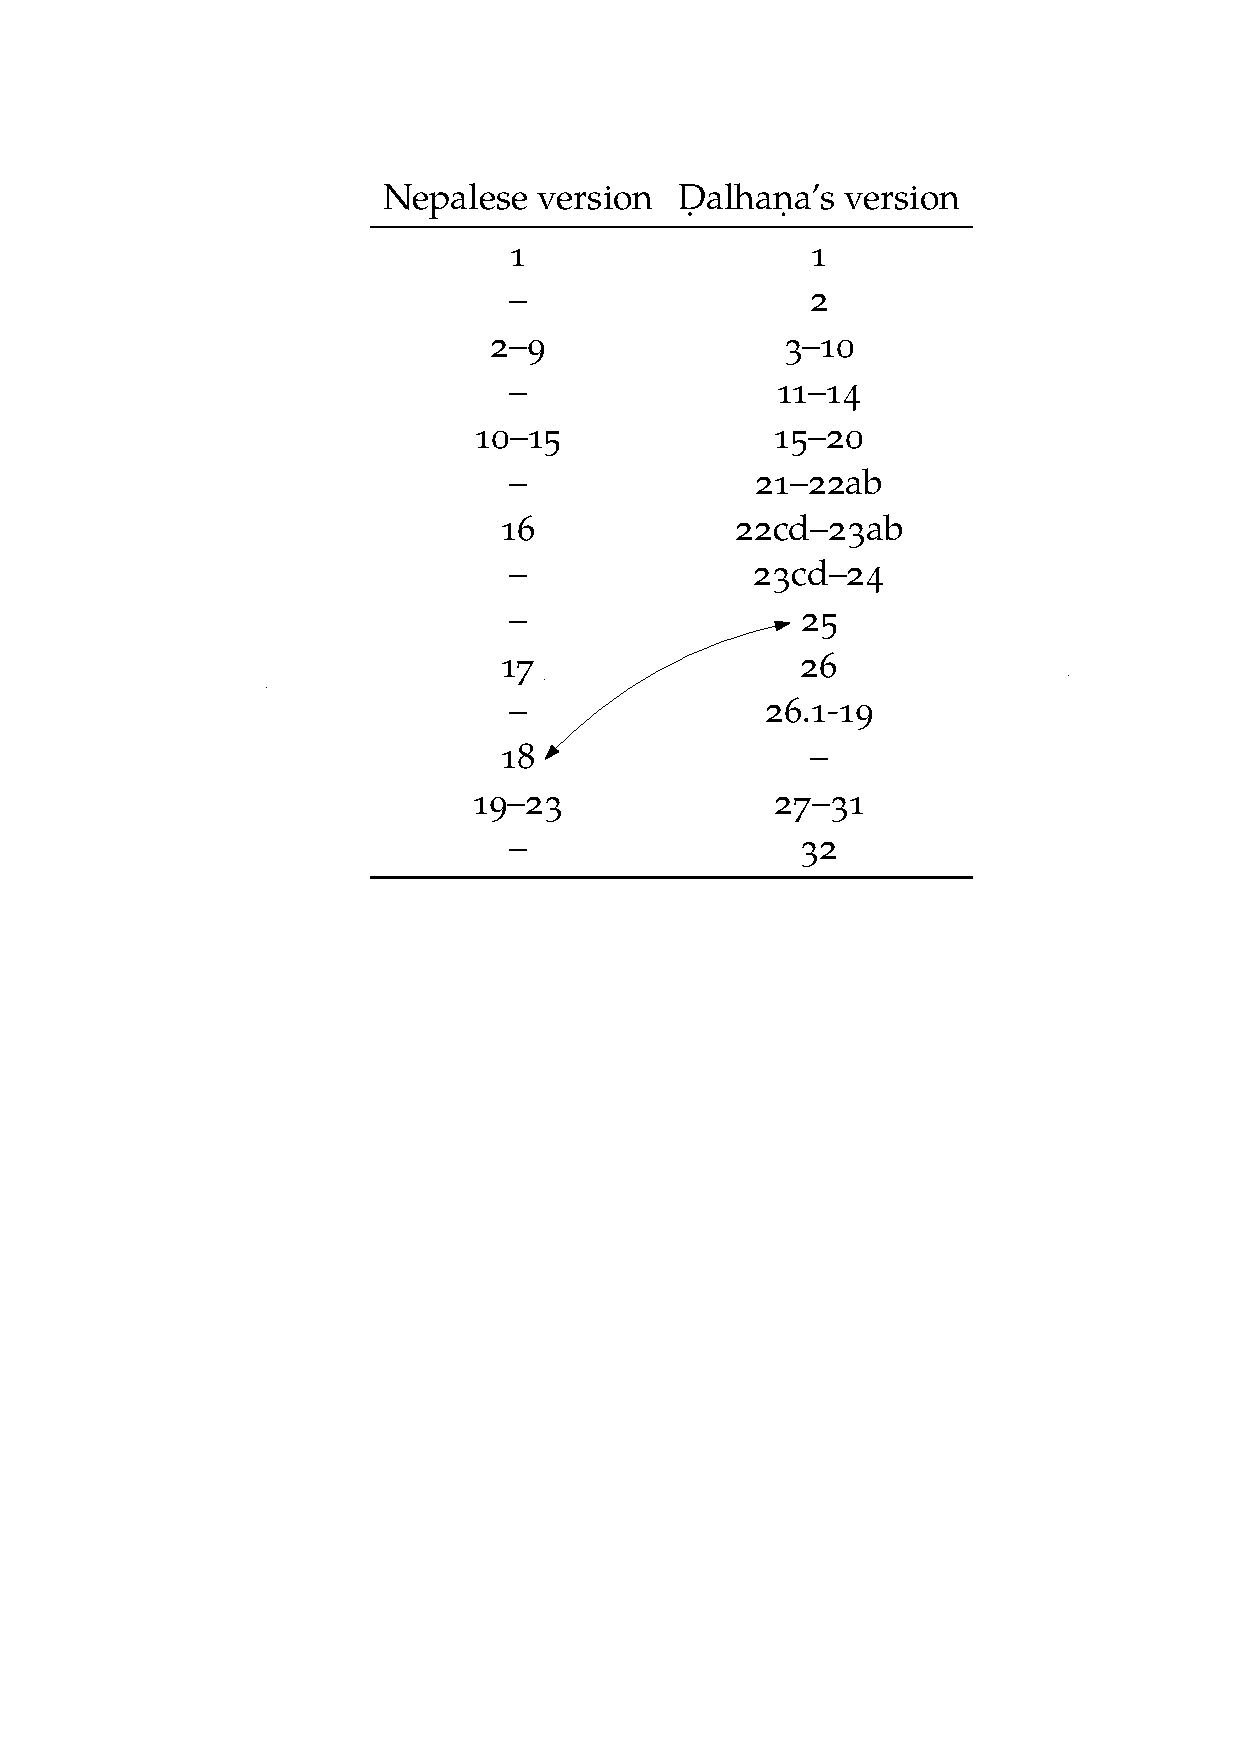
\includegraphics[draft=false,width=\textwidth]{table-of-versions.pdf}
\caption{A Comparison of Verses in 1.16 of the Nepalese and Ḍalhaṇa's Versions}
\end{table}

In Table 1, one can also see that verses 17 and 18 of the Nepalese version were transposed in the redaction of Ḍalhaṇa's version, in which they are 26 and 25 respectively. Although this only occurs once in 1.16, such transposing of verses and even their hemistiches is more prevalent in the redaction of other chapters of the \SS.

Apart from the addition of verses, the redacting of the version known to Ḍalhaṇa involved many small, yet sometimes significant, changes that are summarised below. 

\subsubsection{Changing Spelling, Sandhi and Syntax}
In the majority of cases, efforts were made by redactors to standardise, simplify or improve the language of the Nepalese version. Such changes include the standardising of spelling,\footnote{For example, \emph{pattāṅga} (SS.1.16.21) → \emph{pataṅga} (1.16.29, \cite[81]{vulgate}). For more information on this, see the relevant footnote to the translation.} sandhi,\footnote{or example, \emph{°hastena ṛju} (SS.1.16.2) → \emph{°hastena rju} (1.16.3, \cite[76]{vulgate}).} and verbal forms,\footnote{For example, \emph{unnāmayitvā} (SS.1.16.21) → \emph{prānnamya} (1.16.29, \cite[81]{vulgate}); \emph{avacūrṇayīta} (SS.1.16.21) → \emph{upaharet} (1.16.29, \cite[81]{vulgate}).} as well as interventions to simplify and clarify syntax,\footnote{For example, \emph{śoṇitabahutvanivedanāyāṃ cānyadeśaviddham iti jānīyāt | nirupadravatā taddeśaviddhaliṅgam |} (SS.1.16.3) → \emph{śoṇitabahutvena vedanayā cānyadeśaviddham iti jānīyāt | nirupadravatayā taddeśaviddham iti |} (1.16.4, \cite[76]{vulgate}); \emph{āmatailapariṣekeṇopacaret} (SS.1.16.6) → \emph{āmatailena pariṣecayet} (1.16.7, \cite[77]{vulgate}); \emph{suparigṛhītaṃ} (SS.1.16.10) → \emph{suparigṛhītaṃ ca kṛtvā} (1.16.15, \cite[78]{vulgate}); \emph{anena} (SS.1.16.15) → \emph{snehenaitena} (1.16.20, \cite[79]{vulgate}).} which often involved splitting compounds.\footnote{For example, \emph{yadṛcchāviddhāyāṃ sirāyām} (SS.1.16.4) → \emph{yadṛcchayā viddhāsu sirāsu} (1.16.5, \cite[76]{vulgate}); \emph{dhānyāmlakapālacūrṇaṃ} (SS.1.16.10) → \emph{dhānyāmlaṃ kapālacūrṇaṃ} (1.16.20, \cite[78]{vulgate}).} In some instances, these changes improved the grammar,\footnote{For example, \emph{surāmaṇḍakṣīram} (SS.1.16.10) → \emph{surāmaṇḍaṃ kṣīram} (1.16.15, \cite[78]{vulgate}).} or altered the meaning.\footnote{For example, \emph{kṣīṇālpamāṃsaḥ} (SS.1.16.12) → \emph{kṣīṇo 'lpamāṃsaḥ} (1.16.17, \cite[79]{vulgate}).} However, some prefixes of verbal forms,\footnote{For example, \emph{samvarddhitaḥ} (SS.1.16.8) → \emph{vivarddhitaḥ} (1.16.9, \cite[77]{vulgate}); \emph{niveśya} (SS.1.16.10) → \emph{sanniveśya} (1.16.15, \cite[78]{vulgate}); \emph{avabadhya} (SS.1.16.10) → \emph{ca baddhvā} (1.16.15, \cite[78]{vulgate}).} case endings,\footnote{For example, \emph{māse} (SS.1.16.2) → \emph{māsi} (1.16.3, \cite[76]{vulgate}).} and indeclinables were changed for less apparent reasons.\footnote{For example, \emph{api} (SS.1.16.13) → \emph{vā} (1.16.18, \cite[79]{vulgate}); \emph{ca} (SS.1.16.16) → \emph{tu} (1.16.23, \cite[79]{vulgate}); \emph{tu} (SS.1.16.18) → \emph{ca} (1.16.25, \cite[80]{vulgate}).} There is also a tendency to replace uncommon words with generic ones,\footnote{For example, \emph{mrakṣayet} (SS.1.16.15) → \emph{yojayet} (1.16.20, \cite[79]{vulgate}); \emph{nahyet} (SS.1.16.21) → \emph{baddhvā} (1.16.29, \cite[81]{vulgate}).} add indeclinables,\footnote{For example, [absent]  (SS.1.16.6) → \emph{ca} (1.16.7, \cite[77]{vulgate}); [absent] (SS.1.16.10) → \emph{tatra} (1.16.15, \cite[78]{vulgate}); [absent]  (SS.1.16.12) → \emph{api} (1.16.17, \cite[79]{vulgate}).} omit the verb to be at the end of sentences,\footnote{The words \emph{bhavati} or \emph{bhavanti} are omitted four times in Ḍalhaṇa's version (1.16.10 (twice), 1.16.17 and 1.16.18, \cite[77, 79]{vulgate}).}and introduce verses after a prose passage with the phrase \emph{bhavati cātra}.\footnote{For example, [absent] (SS.1.16.11) → \emph{bhavati cātra} (1.16.16, \cite[79]{vulgate}).} 

% Spelling
% 9. nemī → nemi
% 9. yaṣṭī → yaṣṭi
% 9. kākauṣṭhaḥ → kākauṣṭhakaḥ
% 21. pattāṅga → pataṅga *

%Sandhi
% 2 °hastena ṛju  →  °hastena rju (standardise)*

% Standardising and Simplifying Syntax
% 3.  śoṇitabahutvanivedanāyāṃ cānyadeśaviddham iti jānīyāt | nirupadravatā taddeśaviddhaliṅgam || → śoṇitabahutvena vedanayā cānyadeśaviddham iti jānīyāt || nirupadravatayā taddeśaviddham iti ||*
% 6 āmatailapariṣekeṇopacaret → āmatailena pariṣecayet*

% Clarifying syntax
%15 anena → snehenaitena*

% Splitting compounds
% 4. yadṛcchāviddhāyāṃ	sirāyām	 → 	yadṛcchayā viddhāsu	sirāsu (clarifies syntax)*
% 10. surāmaṇḍakṣīram → surāmaṇḍaṃ kṣīram (improves grammar)*
% 10. dhānyāmlakapālacūrṇañ → dhānyāmlaṃ kapālacūrṇañ*
% 12. kṣīṇālpamāṃsaḥ → kṣīṇo 'lpamāṃsaḥ (changes the meaning)*

% Changing verbs and gerunds
% 2. vyadhayet → vidhyete (perhaps, picking up on karnau)
% 6. kurvīta → dadyāt (middle to active) 
% 7. muñcet → kuryāt
% 9. bandhyā bhavanti → sādhyāḥ
% 10. suparigṛhītaṃ → suparigṛhītaṃ ca kṛtvā ( attempt to improve syntax)*
% 10. upapādya → upadhārya
% 10. sandarśya → sandadhyāt | tato (attempt to simplify the sentence)
% 13. chidyeta → chidyate (opt to pres)
% 15. mrakṣayet → yojayet * (replacing less common words with generic ones)
% 21. nahyet → baddhvā*
% 21. unnāmayitvā → prānnamya (standardise)*
%21 avacūrṇayīta → avacūrṇayet (standardise)*

% Omitting bhavati
% Happens a few times; e.g., 1.16.9 (twice), 1.16.12, 1.16.13

% Changing Prefixes
% 8. samvarddhitaḥ → vivarddhitaḥ*
% 10. niveśya → sanniveśya*
% 10. avabadhya → ca baddhvā*
% 15. marditaṃ → unmarditaṃ*
% 21. unnāmayitvā → prānnamya *

% Changing case endings
% 2. māse → māsi (shift from māsa to mās. Can't see a reason)
% 3. śoṇitabahutvanivedanāyāṃ →  śoṇitabahutvena vedanayā (splitting compounds, but locative of circumstance or condition changed to instrumental of reason. latter is clearer, but not much in it)
% 19. viśleṣitāyām atha nāsikāyāṃ → °tāyās tv nāsikāyāḥ

% changing indeclinables
%13 anyathā → ato 'nyathā
% 13 api → vā*
% 15 tataḥ → ataḥ
% 16 ca → tu*
% 18 tu → ca*
% 19 atha → tu
% 23 vai → syāt

% Adding indeclinables
% 10 [absent] → tatra
% 6 [absent] → ca
% 9 [absent] → tu
% 10 [absent] → ca
% 12 [absent] → api
% 14 [absent] → vā

% Omitting indeclinables
% 9 tatra → [absent]
% 9 ca → [absent]

%Adding bhavati cātra before verses.

% Not sure
% 2
% kṛtamaṅgalaṃ svastivācanan → kṛtamaṅgalasvastivācanan (the latter makes better sense, but could have been original, in my opinion, or an attempt to better integrate a gloss that had become part of the text.)
% abhisāntvayamānaḥ → abhisāntvayan (shift from Pres Pass Part to Pres Act Part) % It seems only the latter is correct in the given context. So, it could be just an error in the NV. Emend or Change translation!!! 
% % 10. agropaharaṇīyāt appears to be an error in the NV that needs to be emended.

\subsubsection{Changing Technical Terms}
There is evidence of standardising and altering technical terminology in subsequent versions of the \SS. Two examples of this in SS.1.16 are the terms for \se{bandha}{joins} and \se{vadhra}{a slice of flesh}. The Nepalese version uses three terms for \se{bandha, sandhāna, sandhi}{joining} splits in the ear flaps and the flesh of nose. Redactors of subsequent versions appear to have tried to standardise this terminology by replacing \emph{sandhāna} and \emph{sandhi} with \emph{bandha} in prose passages.\footnote{For example, \emph{pañcadaśasandhānākṛtayaḥ} (SS.1.16.9) → \emph{pañcadaśabandhākṛtayaḥ} (SS.1.16.10, \cite[77]{vulgate}); \emph{daśakarṇasandhivikalpāḥ} (SS.1.16.9) → \emph{karṇabandhavikalpāḥ} (SS.1.16.10, \cite[77]{vulgate})} However, the use of the term \emph{sandhāna} was retained in verses, perhaps because of the metrical challenges of making such a change. Also, the names of joins which incorporate \emph{sandhāna} and \emph{sandhi} remained the same.\footnote{These names are \emph{nemīsandhānaka}, \emph{kapāṭasandhika}, and \emph{ardhakapāṭasandhika} in SS.1.16.9.}

The Nepalese version (SS.1.16.20,23) contains the rather obscure term \emph{vadhra} for the slice of flesh that a surgeon cuts from the cheek in order to construct a new nose. Modern dictionaries define \emph{vadhra} as a leathern strap (\cite[1385]{apte-prac}, \cite[917]{moni-sans}) or a slice of bacon (\cite[917]{moni-sans}),\q{refs} the latter of which is more indicative of its meaning in the Nepalese version. This word was written out of subsequent versions,\footnote{\emph{vadhram} (SS.1.16.20) → \emph{baddham} (SS.1.16.28, \cite[81]{vulgate}) and \emph{tadvadhraśeṣaṃ} (SS.1.16.23) → \emph{tad ardhaśeṣaṃ} (SS.1.16.31, \cite[81]{vulgate}).} and it was not mentioned as an alternative reading by either Cakrapāṇidatta or Ḍalhaṇa, which suggests that its use and meaning may not have been known to them. However, \emph{vadhra} was used by the author of the \emph{Aṣṭāṅgahṛdayasaṃhitā} (\Ah{Utt.18.62}{841}) in the context of rhinoplasty, so it likely to be the correct reading in the Nepalese version. 

% bandha
% 1. athātaḥ karṇavyadhavidhim vyākhyāsyāmaḥ  → athātaḥ karṇavyadhabandhavidhim adhyāyaṃ (prose)
% sandhāna in all version (verse)
% 9. pañcadaśasandhānākṛtayaḥ (SS.1.16.9) → pañcadaśabandhākṛtayaḥ (SS.1.16.10) (sandhāna is reflected in the name nemisandhānaka, which is in all versions) 
% 9. daśakarṇasandhivikalpāḥ → karṇabandhavikalpāḥ (sandhi is in many of the names, bandha is not)
% 10. (twice) bandha in all versions
% 17 karṇabandha in all versions
% 19 & 23. sandhāna accepted in all versions + 32 in DV. (verse)
% 20. sādhubaddham → sādhubandhaiḥ (verse)
%
% vadhra 
% 20 vadhram → baddham 
% 21 susīvitaṃ → susaṃhitaṃ
% 23 tadvadhraśeṣaṃ → tad ardhaśeṣaṃ

\subsubsection{Augmenting the Text}

Apart from adding whole passages and verses (as seen in Table 1), redactors of subsequent versions augmented the text by expanding existing compounds and inserting new compounds and words. Within the microcosm of 1.16, adjectives and adverbs were inserted to clarify statements,\footnote{For example, \emph{chidre} (SS.1.16.2) → \emph{chidra ādityakarāvabhāsite} (1.16.3, \cite[76]{vulgate}); [absent] (SS.1.16.2) → \emph{śanaiḥ śanaiḥ} (1.16.3, \cite[76]{vulgate});  [absent] (SS.1.16.3) → \emph{āśu} (1.16.5, \cite[77]{vulgate}).} and phrases added to elaborate on diseases and treatments.\footnote{For example, \emph{dhātryaṅke} (SS.1.16.2) → \emph{dhātryaṅke kumāradharāṅke vā} (1.16.3, \cite[76]{vulgate}); [absent] (SS.1.16.2) → \emph{bālakrīḍanakaiḥ pralobhya} (1.16.3, \cite[76]{vulgate});  [absent] (SS.1.16.3) → \emph{picuvartiṃ praveśayet} (1.16.5, \cite[77]{vulgate}).} In particular, the characteristics and number of symptoms of a disease, as well as their reasons for arising, tend to increase in subsequent versions. For example, the Nepalese version (SS.1.16.5) says that the wick in a newly pierced ear should be removed because of aggravated humours or a culpable piercing whereas the version known to Ḍalhaṇa (1.16.6, \cite[77]{vulgate}) includes two further reasons, namely, because of piercing with a painful, crooked and unrecommended needle or because of a wick that is too thick. Some of the split ear flaps in Ḍalhaṇa's version have additional characteristics,\footnote{For example, \emph{pīṭhopamapālir nirvedhimaḥ} (SS.1.16.9) → \emph{pīṭhopamapālir ubhayataḥ kṣīṇaputrikāśrito nirvedhimaḥ} (1.16.10, \cite[77]{vulgate}); \emph{itarālpapāliḥ saṃkṣiptaḥ} (SS.1.16.9) → \emph{utsannapālir itarālpapāliḥ saṃkṣiptaḥ} (1.16.10, \cite[77]{vulgate}); \emph{tanuviṣamapāliḥ} (SS.1.16.9) → \emph{tanuviṣamālpapāliḥ} (1.16.10, \cite[77]{vulgate}).} and a list of four symptoms associated with incurable joins in the Nepalese version (SS.1.16.19) was increased to six in Ḍalhaṇa's version (1.16.10, \cite[77]{vulgate}). Also, models of classifying symptoms were introduced in subsequent versions. For example, the Nepalese version (SS.1.16.4) lists the symptoms of mistakenly piercing a duct in the ear whereas the version known to Ḍalhaṇa (1.16.5, \cite[76–77]{vulgate}) classifies these symptoms according to three ducts called \emph{kālikā}, \emph{marmarikā} and \emph{lohitikā}, which results in some repetition of the symptoms mentioned.\footnote{In Ḍalhaṇa's version  (1.16.5, \cite[76–77]{vulgate}), the symptoms of \se{jvara}{fever} and \se{vedanā}{pain} are repeated. This repetition does not occur in the Nepalese version. It is possible that this classification was not in the version of the \SS\ known to Cakrapāṇidatta (1.16.4, \cite[126]{acar-1939}) because he mentions that some read classifications of ducts at this point in the text and he cites verses from Bhoja on \emph{kālikā}, \emph{marmarikā} and \emph{lohitikā}, but he does not gloss or comment on the passage known to Ḍalhaṇa.}

% Supplementary compounds and phrases for Adding Information
% This is done by expanding compounds, inserting new compounds and adverbs and adding verses and passages.
% 
% 1. karṇavyadhavidhim → karṇavyadhabandhavidhim (foregrounding the term bandha)
% 2
% dhātryaṅke → dhātryaṅke kumāradharāṅke vā (elaborating on treatment)
% upaveśyābhisāntvayamānaḥ → upaveśya bālakrīḍanakaiḥ pralobhyābhisāntvayan (elaborating on treatment)
% chidre → chidra ādityakarāvabhāsite (clarifying technical term)
% [absent] → śanaiḥ śanaiḥ (clarifying treatment)
% [absent] → picuvartiṃ praveśayet (elaborating on treatment)
% 4 
% [absent] →  kālikāmarmarikālohitikāsūpadravā and dividing the adverse affects according to kālikā, marmarikā and lohitikā. Repetition of vedanā and jvara in this process.(discussed in footnote). teṣu yathāsvaṃ pratikurvīt || (adding symptoms, perhaps with a view to managing them more effectively, according to the type of vein pierced).
% 5
% [absent] → kliṣṭajihmāpraśastasūcīvyadhād gāḍhataravartitvād (adding reasons)
% [absent] → yatra saṃrambho vedanā vā bhavati (adding information about the treatment)
%  [absent]  → āśu (clarifies the treatment)
%  [absent] → tāvad yāvat surūḍha iti (until it is well healed - clarifies the treatment)
%9
% pīṭhopamapālir nirvedhimaḥ → pīṭhopamapālir ubhayataḥ kṣīṇaputrikāśrito nirvedhimaḥ (adding characteristics)
% itarālpapāliḥ saṃkṣiptaḥ → utsannapālir itarālpapāliḥ saṃkṣiptaḥ (adding characteristics)
% tanuviṣamapālir → tanuviṣamālpapālir (adding characteristics)
% baddheṣv api dāhapākasrāvaśophayuktā	na siddhim upayānti → tu śophadāharāgapākapiḍakāsrāvayuktā	na siddhim upayānti (adding symptoms)
% 10
% surāmaṇḍodakābhyāṃ → surāmaṇḍoṣṇodakābhyāṃ (adding characteristics of an ingredient)
% 12
% gāḍhapākarāgavān → dāhapākarāgavedanāvān (adding symptoms)

% Additional Verses and Passages (table 1)
% For passages, see subsub on Elaborating on Treatments.
%  [absent] → 16.11–14 (verses)
%  [absent] → 21–22ab, 23cd–24
%  [absent] → 26.1 – 26.19
%  [absent] → 32

\subsubsection{Transposing Words, Verses and Passages}
A close comparison of the Nepalese version with subsequent ones reveals changes in the order of words, sentences and verses. Examples of such transpositions occur in SS.1.16. In most cases, the changes in word order are insignificant and may be result of different preferences in syntax or even scribal eye-brain-hand miscommunication.\footnote{For example, \emph{aṇusthūla°} (SS.1.16.9) → \emph{sthūlāṇu°} (1.16.10, \cite[77]{vulgate}); \emph{tatraite daśakarṇa°} (SS.1.16.9) → \emph{tatra daśaite karṇa°} (1.16.10, \cite[77]{vulgate}); \emph{nātigāḍhan nātiśithilaṃ sūtreṇāvabadhya} (SS.1.16.9) → \emph{sūtreṇānavagāḍhaman atiśithilaṃ ca baddhvā} (1.16.10, \cite[77]{vulgate}); \emph{pūrvan dakṣiṇaṃ kumārasya vāmaṅ kanyāyāḥ | pratanuṃ sūcyā bahalam ārayā } (SS.1.16.2) → \emph{pratanukaṃ sūcyā bahalam ārayā | pūrvaṃ dakṣiṇaṃ kumārasya vāmaṅ kanyāyāḥ} (1.16.3, \cite[76]{vulgate}).} However, the transposition of verses and passages is usually the result of efforts at redacting the text to add new material. A good example of this is the transposition of SS.1.16.17 and SS.1.16.18 in the Nepalese version to 1.16.26 and 1.16.25, respectively, in Ḍalhaṇa's. It seems that this transposition may have resulted from the insertion of new verses 1.16.23cd–24 and 1.16.26.1–19 in the latter.

% Words
% 9. aṇusthūla° → sthūlāṇu°
% 9. tatraite daśakarṇa° → tatra daśaite karṇa°
%  10. nātigāḍhan nātiśithilaṃ sūtreṇāvabadhya → sūtreṇānavagāḍhaman atiśithilaṃ ca baddhvā
% Passages
% 2. pūrvan dakṣiṇaṃ kumārasya vāmaṅ kanyāyāḥ | pratanuṃ sūcyā bahalam ārayā || → pratanukaṃ sūcyā bahalam ārayā || pūrvaṃ dakṣiṇaṃ kumārasya vāmaṅ kanyāyāḥ ||
% Verses
%17 and 18 → 26 and 25

%
\subsubsection{Redacting Recipes and Elaborating on Treatments}
Some of the additional text in subsequent versions of the \SS\ introduces new ingredients in recipes and different procedures in treatments. In many instances, the new material merely clarifies or elaborates on the original but sometimes it changes the recipe or treatment significantly. An example of a suppletion that clarifies the text of the Nepalese version can be seen in 1.16.3 of Ḍalhaṇa's version (\cite[76]{vulgate}), which contains a statement that the physician should insert a wick of cotton after the ear has been pierced.\footnote{For example, [absent] (SS.1.16.2) → \emph{picuvartiṃ praveśayet} (1.16.3, \cite[76]{vulgate}).} This statement anticipates the instructions in the the Nepalese version (SS.1.16.5–6) on removing the wick because of aggravated humours and replacing the wick with a thicker one every three days. In this case, the additional statement of Ḍalhaṇa's version elucidates the role of the wick in the procedure of piercing the ear. 

A similar clarification occurs in 1.16.18 of Ḍalhaṇa's version (\cite[79]{vulgate}), which reiterates the cure for an ear tainted by a humour that was described in 1.16.7 (= SS.1.16.6). The reiteration is quite apt because it follows a passage  (1.16.17, \cite[79]{vulgate} = SS.1.16.12) that outlines the various symptoms of ear disease arising from each of the three humours. The author of the Nepalese version probably assumed that, after reading SS.1.16.12, the reader would refer back to SS.1.16.6 for the cure of an ear affected by a humour. However, in Ḍalhaṇa's version, the treatment is reiterated at 1.16.18.

In  Ḍalhaṇa's version of 1.16, there are two instances in which ingredients were added to recipes of medicines in the Nepalese version. The first is the recipe of an anointment that should be applied to a pierced ear that has not healed. In Ḍalhaṇa's version (1.16.7, \cite[77]{vulgate}) the recipe was rewritten to include sesame seeds.\footnote{\emph{yavamadhukamañjiṣṭhāgandharvahastamūlair madhughṛtapragāḍhair ālepayet} (SS.1.16.5) → \emph{madhukairaṇḍamūlamañjiṣṭhāyavatilakalkair madhughṛtapragāḍhair ālepayet} (1.16.7, \cite[77]{vulgate}).} A more significant change occurs in another recipe for an admixture of an oil that is supposed to be rubbed into a healthy ear to enlarge it. Ḍalhaṇa's version (1.16.7, \cite[77]{vulgate}) of the admixture has five additional ingredients, namely, \se{apāmārga}{prickly chaff-flower}, \se{aśvagandhā}{Withania}, \se{kṣīraśuklā}{giant potato}, \se{madhuravarga}{ the `sweet' savour}\footnote{The items which exemplify the `sweet' savour \label{kakolyadi} (\emph{madhuravarga}) are enumerated at SS.1.42.11.} and `milk flower' (\emph{payasyā}  $\rightarrow$ \emph{vidāri}\footnote{Pueraria tuberosa (Willd.) DC. (ADPS 510, IMP 1.792f., AVS 4.391; not Dymock 1.424f. See GJM supplement 444, 451, IMP 1.187, but IMP 3.1719 = Ipmoea mauritiana, Jacq.). }). It also has \se{vidārigandhā}{beggarweed} instead of \se{vidāri}{milk flower}.\footnote{\emph{arkālarkabalātibalānantāvidārīmadhukajalaśūkaprativāpan tailam pācayitvā } (SS.1.16.14) → \emph{arkālarkabalātibalānantāpāmārgāśvagandhāvidārigandhākṣīraśuklājalaśūkamadhuravargapayasyāprativāpaṃ tailam vā pācayitvā} (1.16.19, \cite[79]{vulgate}).} This method of redacting a recipe of Nepalese version appears to be somewhat typical in so far as most of the ingredients of the original were retained and new ones simply added. \q{Perhaps, Dr Madhu could add a comment on whether these additional ingredients would change the effects of the treatment in any significant way?}


% 2. [absent] → picuvartiṃ praveśayet (adding a cotton wick after piercing the ear of a boy or girl)
% 5. yavamadhukamañjiṣṭhāgandharvahastamūlair	madhughṛtapragāḍhair ālepayet → madhukairaṇḍamūlamañjiṣṭhāyavatilakalkair madhughṛtapragāḍhair ālepayet (adding the ingredient tila)
% 5  [absent] → tāvad yāvat surūḍha iti [...] vidhānaṃ tu pūrvoktam eva || (until it is well healed [... One should pierce it again by] the method taught earlier- clarifies the treatment)
% 13.  [absent] → āmatailena trirātraṃ pariṣecayet trirātrāc ca picuṃ parivartayet | (extending the treatment)
% 14. arkālarkabalātibalānantāvidārīmadhukajalaśūkaprativāpan tailam pācayitvā →	arkālarkabalātibalānantāpāmārgāśvagandhāvidārigandhākṣīraśuklājalaśūkamadhuravargapayasyāprativāpaṃ tailam vā	pācayitvā (adding ingredients to an oil)
% additional apāmārga, aśvagandhā, kṣīra, 

